

% ======================================================================
% == Appendix
% ======================================================================

% ## Captionstyle
% > Reset reference counters of figs, tabs, so each chapter starts at 1
\setcounter{figure}{0}
\setcounter{table}{0}
% > Change figure caption from "Figure" to "Appendix Figure"
\captionsetup[figure]{labelformat=appendixfigure} % > Reference in Caption


% == Blank page ========================================================
% > Make a page to mark start of appendix
\markboth{Appendix}{}
\unnsection{Appendix}



% == Contributions to Research Projects ================================
\markboth{Appendix}{: Author Contributions}
\addpdf{Author Contributions to Research Projects}{APPENDIX/Statement_on_ind_author_contributions_4-2022.pdf}
\newpage


% == Contributions to Figures and Tables ===============================
\addpdf{Author Contributions to Figures and Tables}{APPENDIX/Statement_of_individual_author_contributions_to_figures_tables_4-2022.pdf}
\newpage



% == Class Diagramm of plotastic =======================================
\def\mytitle{Class Diagram of \texttt{plotastic}}
\unnsubsection{\mytitle}
\vspace{-\vfull}
\markboth{Appendix}{: \mytitle}

% > Save re-used text in a macro
\def\umlconvention{Arrow shapes follow the UML (unified modeling
    language): A hollow triangle indicates inheritance (\textit{``is~a''}) and a
    filled diamond indicates composition (\textit{``has~a''}). }

% ## Upper part of Diagram
\def\mycap{ \textbf{Class diagram of \texttt{plotastic} (upper part):} The
    architecture of \texttt{plotastic} begins with classes that are related to
    handling a \texttt{pandas.DataFrame} object which stores the data, and defining
    dimensions to group the data (y, x, hue, col, row). This diagram ends with the
    classes \texttt{SubPlot} and \texttt{StatTest} and is continued on the next
    page. \umlconvention }
\begin{figure}[H]
    \centering
    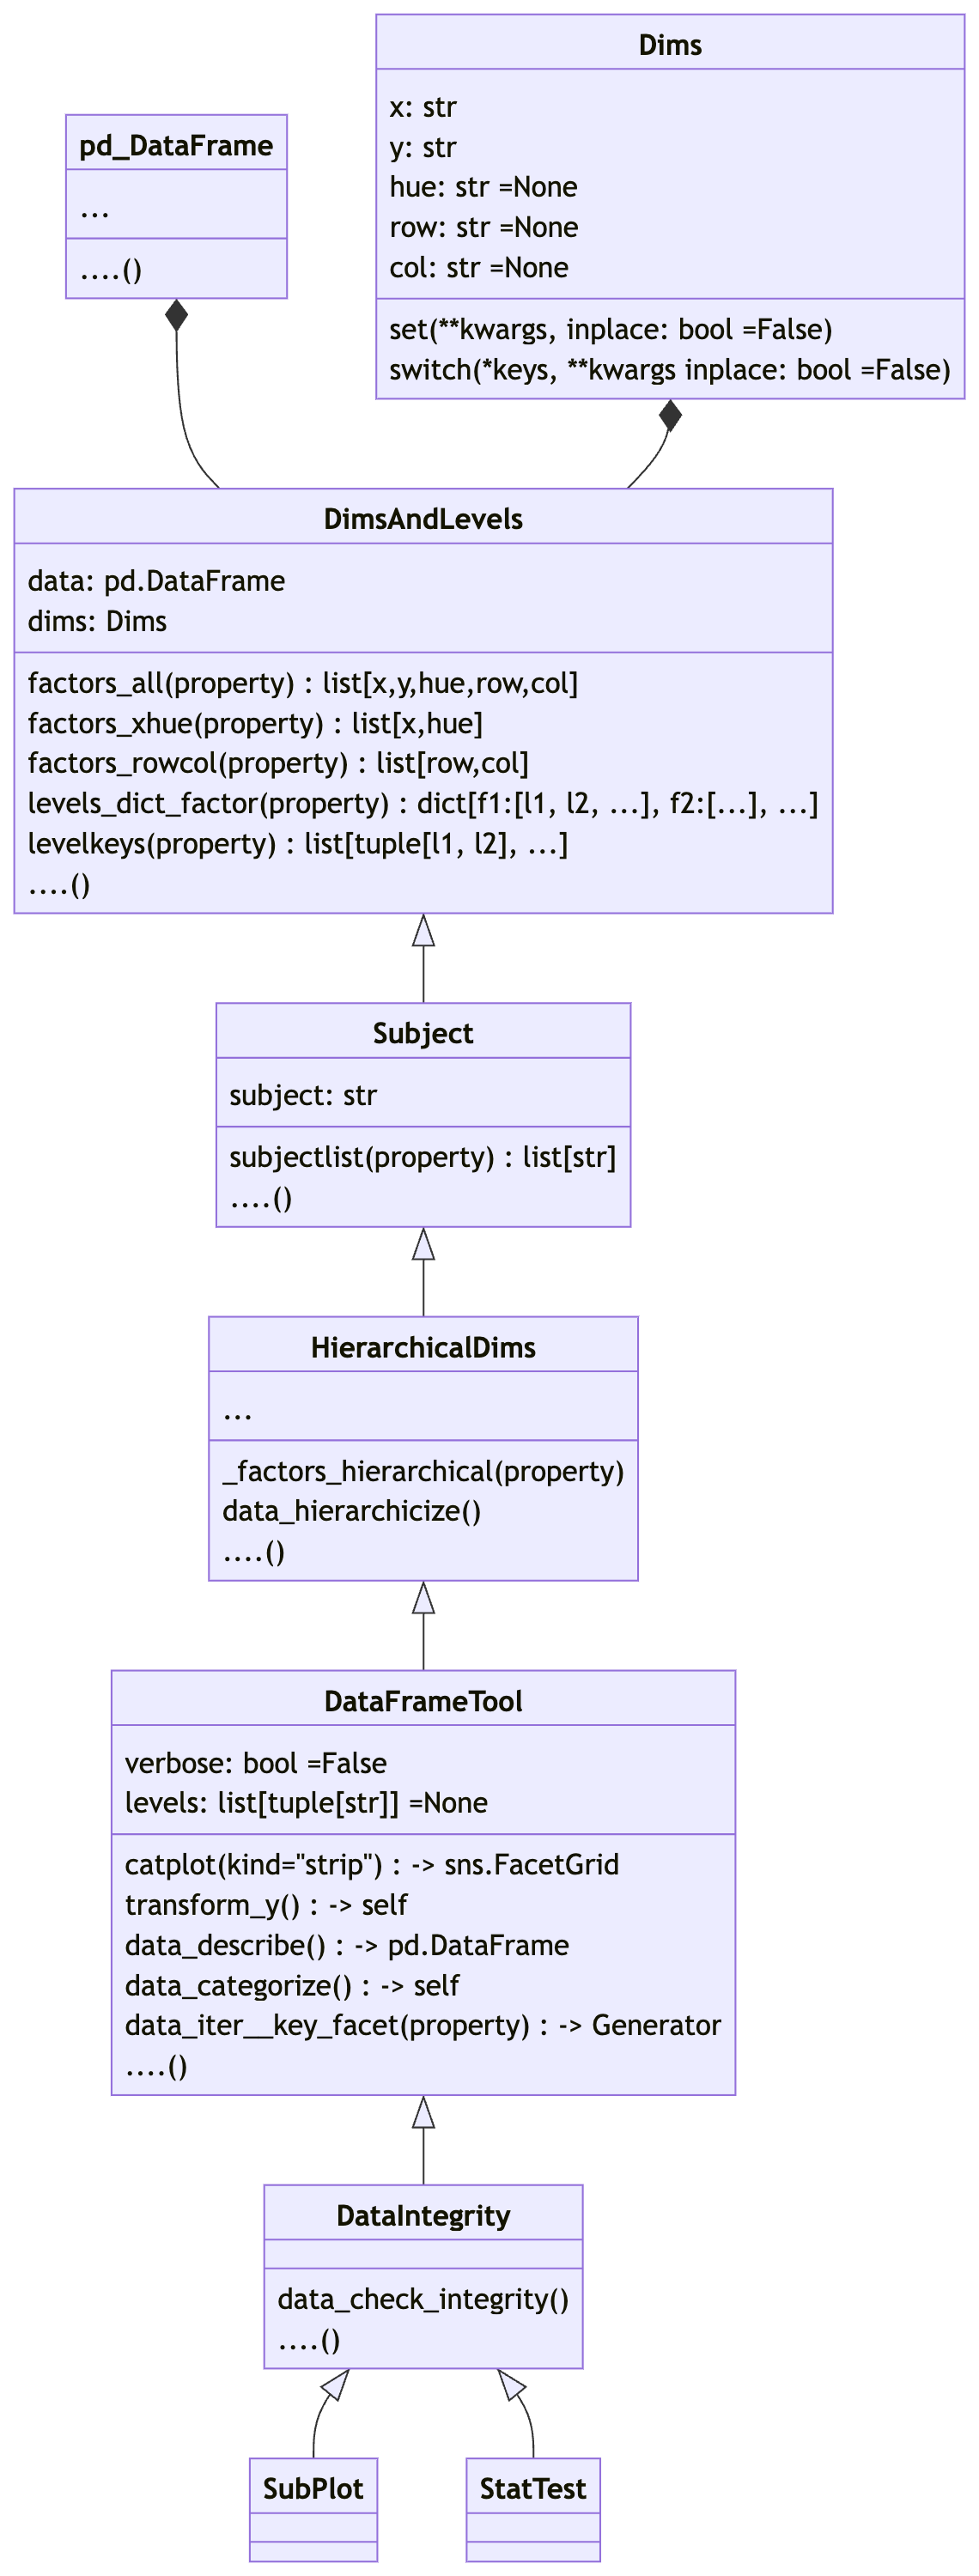
\includegraphics[scale=.18]{APPENDIX/classdiagr_dataframe.png}
    \caption{\mycap}
    \label{fig:classdiagr}
\end{figure}
\newpage

\setcounter{figure}{0} % > Reset figure counter
% > Lower part of Diagram
\def\mycap{\textbf{(continued)} The architecture of \texttt{plotastic}
    continues after the class \texttt{DataIntegrity} with classes for plotting
    (\texttt{SubPlot}) and statistical testing (\texttt{StatTest}) and end with
    the class \texttt{DataAnalysis}, which serves as the main user interface.
    \umlconvention }
\begin{figure}[H]
    \centering
    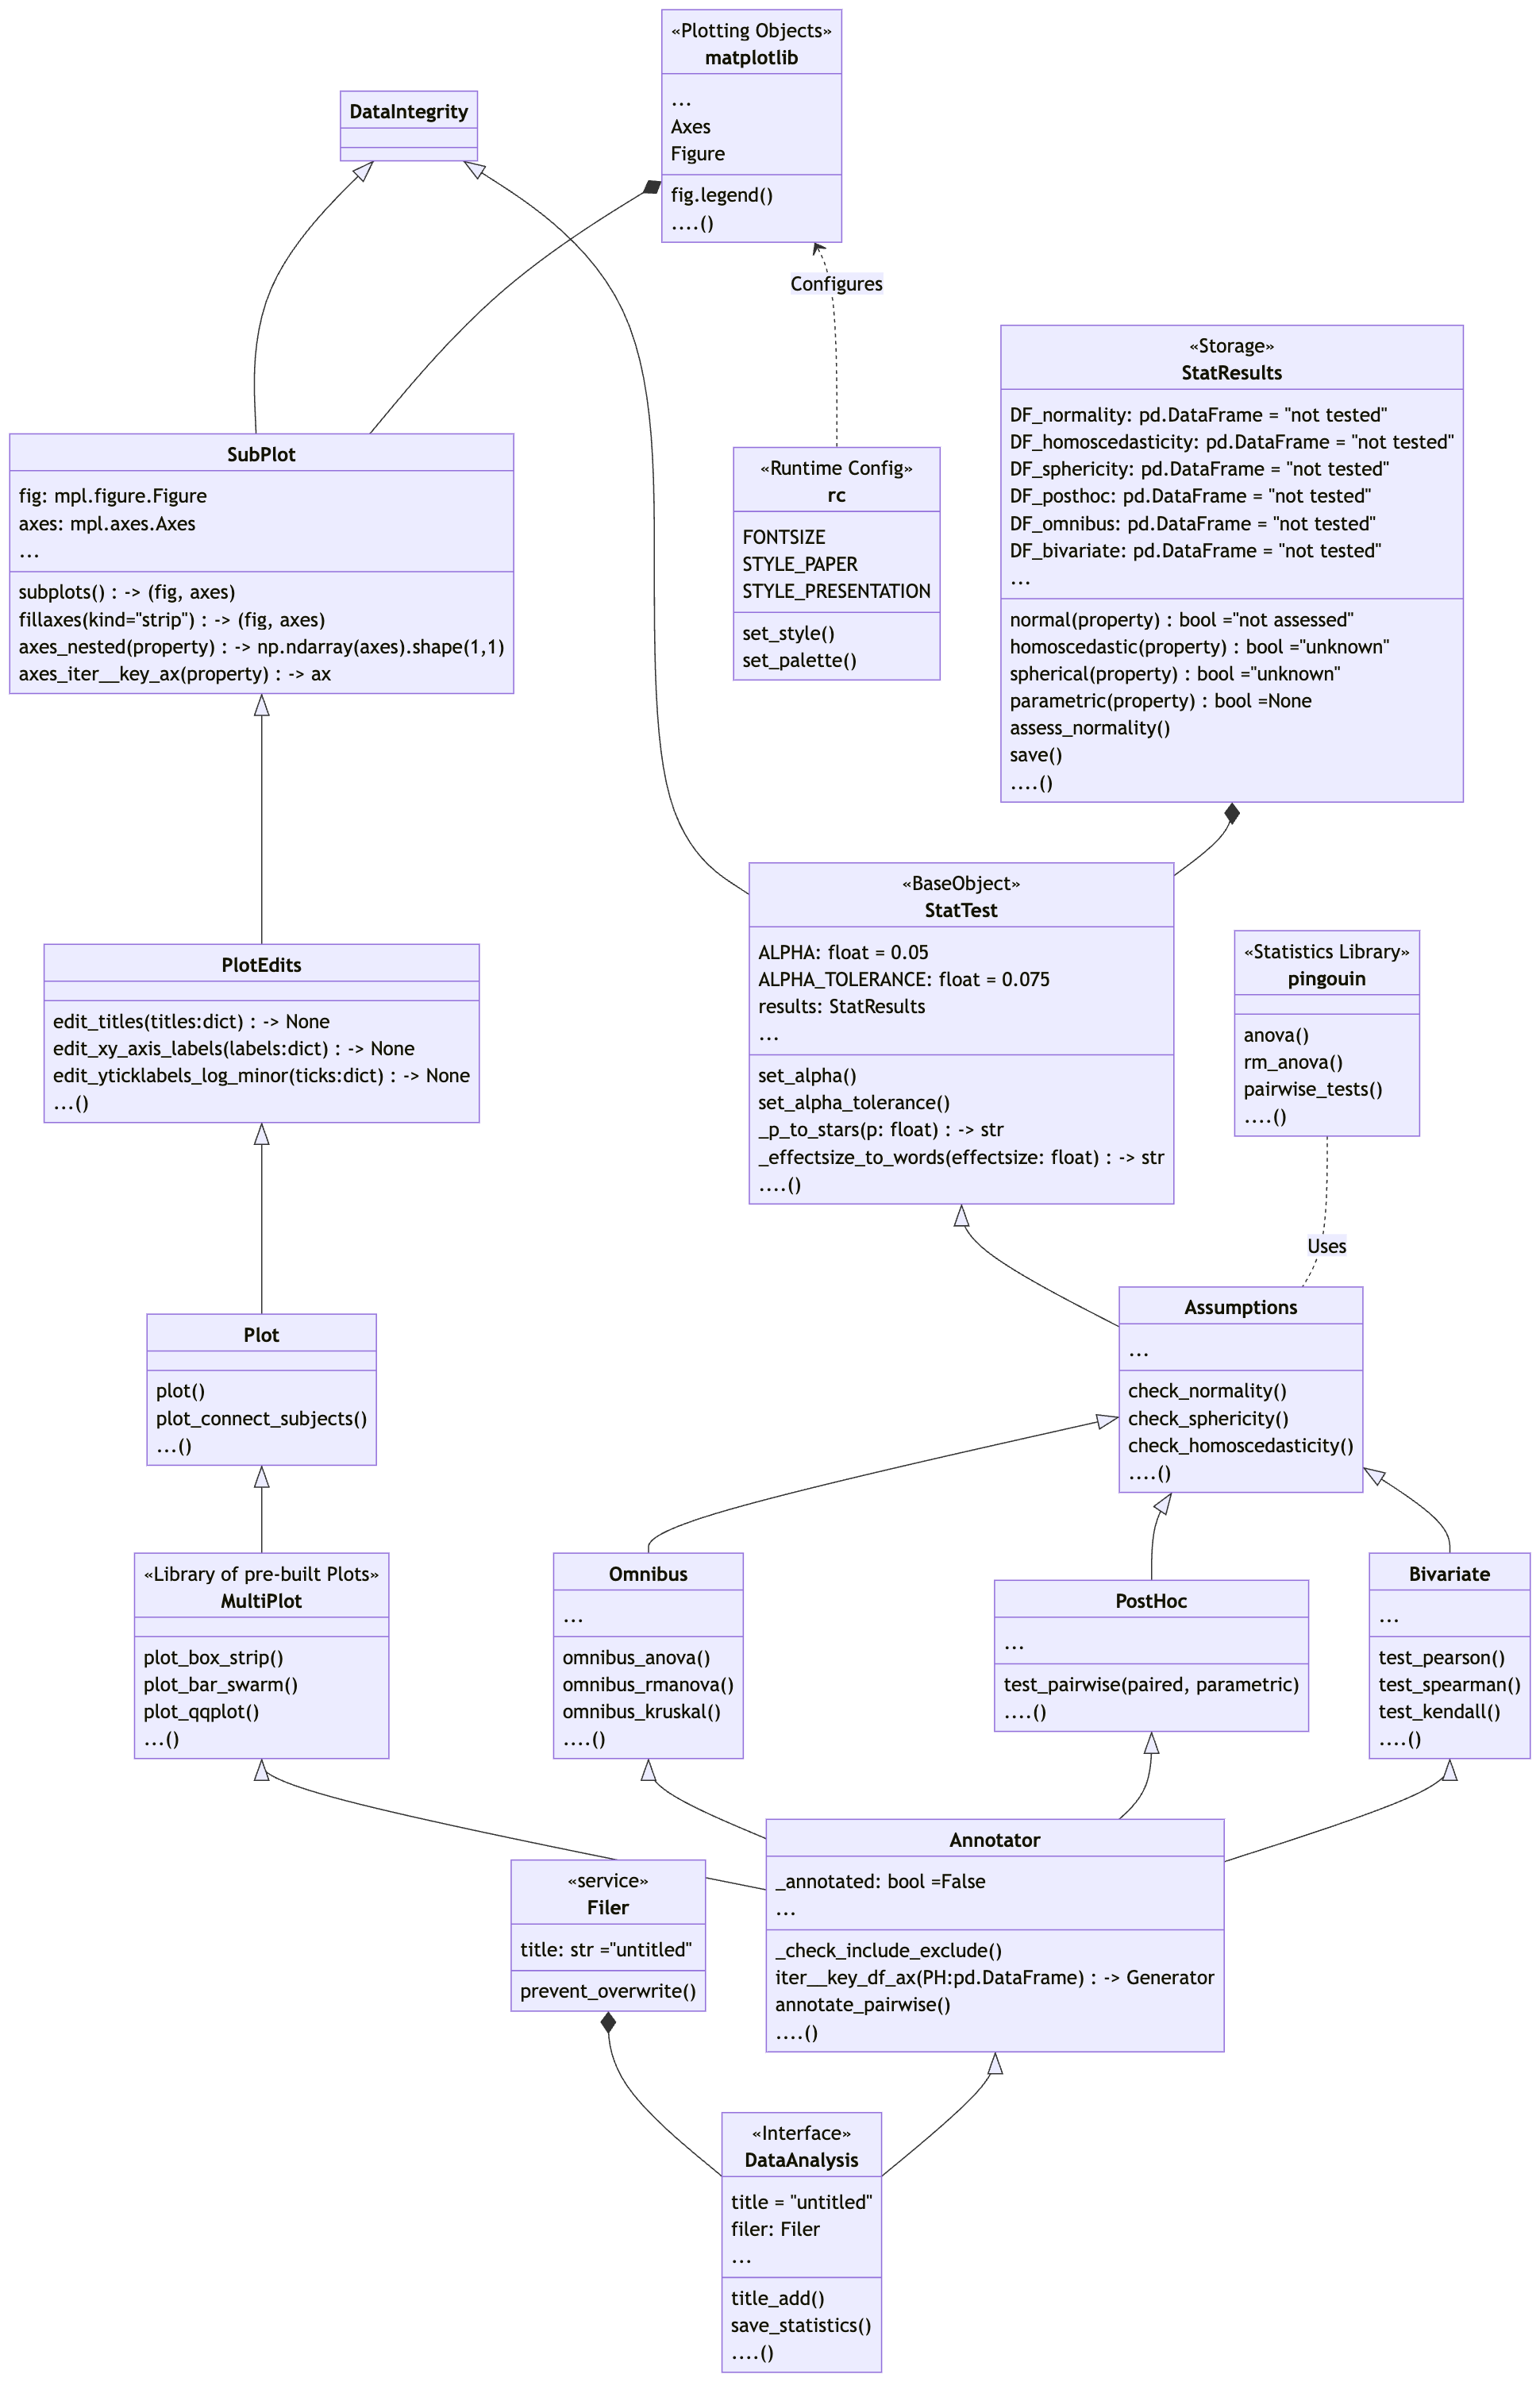
\includegraphics[scale=.20]{APPENDIX/classdiagr_plot+stats.png}
    \caption{\mycap}
\end{figure}



% == Readme from plotastic (PyPi) ======================================
% > Make an empty page with the section title
\def\mytitle{Readme of \texttt{plotastic}}
\markboth{Appendix}{: \mytitle}
\subsection*{\mytitle}
\ %
The following pages are the \texttt{README.md} of \texttt{plotastic} found in
the Python Package Index (PyPi) (\url{pypi.org/project/plotastic}), and on
GitHub (\url{github.com/markur4/plotastic}).

\addpdf[.93]{\mytitle}{APPENDIX/README_pypi.pdf}
\newpage




% == Example Analyses plotastic =======================================
